The projections, connections, and growth cone (GC) morphology of developing axons can be visualized by anterograde labeling with lipophilic dyes \cite{little2009specificity,bielle2011emergent}.
Here, we use the mouse visual system, a classic model for studying neural circuitry development, to demonstrate the advantages of clearing the mouse brain with \emph{Clear\textsuperscript{T}} in preserving lipophilic fluorescent dye labeling.
We anterogradely labeled retinal ganglion cell (RGC) axons in embryonic day (E) 14.5 embryos with DiI and treated embryos with \emph{Clear\textsuperscript{T}}, Sca\emph{l}eA2 or BABB for 1 day.
DiI labeling of retinal axons in the optic nerve and chiasm was preserved after treatment with \emph{Clear\textsuperscript{T}}, but treatment with either Sca\emph{l}eA2 or BABB degraded the fluorescent signal. %(Figure~\ref{ClearT\_SFig2}A).
\begin{figure}[hbtp]
    \begin{center}
        \includegraphics{Figures/ClearT_SFig2.pdf}
        \caption[DiI and CTB labeling is maintained in axons treated with \emph{Clear\textsuperscript{T}} and \emph{Clear\textsuperscript{T2}}.]
        {DiI and CTB labeling is maintained in axons treated with \emph{Clear\textsuperscript{T}} and \emph{Clear\textsuperscript{T2}}.
        A) DiI labeling of E14.5 retinal axons was preserved with \emph{Clear\textsuperscript{T}} and \emph{Clear\textsuperscript{T2}} treatment, but not with Sca\emph{l}eA2 and BABB.
        B) CTB labeling of retinal axons in the dLGN at P6 was maintained with \emph{Clear\textsuperscript{T}}, \emph{Clear\textsuperscript{T2}}, and BABB, but labeling was barely visible in Sca\emph{l}eA2.
        Moreover, BABB-treated tissue shrunk considerably: the surface area of the section after BABB treatment, normalized to pre-cleared sections, was 0.50$\pm$0.02 (mean $\pm$ s.e.m.), n=4 sections; P<0.01, Student’s t-test.
        Scale bars: 100$\mu$m.
        }
        \label{ClearTSFig2}
    \end{center}
\end{figure}

We then examined DiI-labeled RGC axons in cleared tissue at the optic chiasm at E15.5. % (Figure~\ref{ClearT\_Fig2}A).
The DiI-labeled retinal projection was not visible prior to clearing, but could be seen through both dorsal and ventral aspects of the cleared head, with jaw and tongue removed but skin and skull intact. % (Figure~\ref{ClearT\_Fig2}A).
We examined the resolution of fine morphological detail of DiI-labeled axons and GCs in the proximal ipsilateral optic tract at E14.5 before and after clearing. % (Figure~\ref{ClearT\_Fig2}B).
The number and resolution of DiI labeled axons and GC processes (e.g. filopodia and lamellopodia) were markedly increased after clearing with \emph{Clear\textsuperscript{T}}.% (Figure~\ref{ClearT\_Fig2}B).
Furthermore, E18.5 DiI-labeled RGC axons in the thalamus and superior colliculus were not visible before clearing when imaged from the midline of parasagittal hemisections, but the full tract was distinctly visible after clearing with \emph{Clear\textsuperscript{T}}, even through a depth of ~1mm. %  (Figure~\ref{ClearT\_Fig2}C).
\begin{figure}[hbtp]
    \begin{center}
        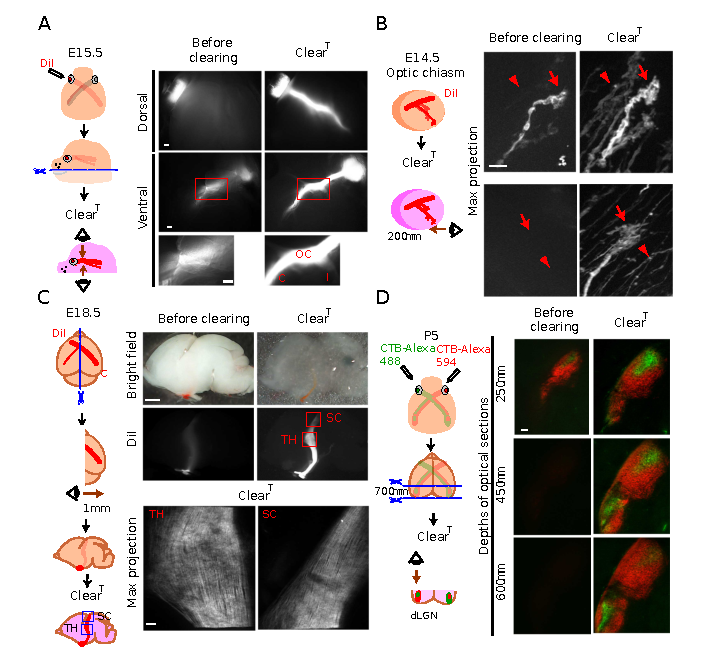
\includegraphics{Figures/ClearT_Fig2.pdf}
        \caption[Retinal axon projections in brain tissue cleared with \emph{Clear\textsuperscript{T}}.]
        {Retinal axon projections in brain tissue cleared with \emph{Clear\textsuperscript{T}}.
        A) E15.5 eye was labeled with DiI, the jaw and tongue were cut away and the head was cleared with \emph{Clear\textsuperscript{T}}.
        DiI-labeled contralateral (C) and ipsilateral (I) retinal axons and optic chiasm are detected in both dorsal and ventral views after clearing with \emph{Clear\textsuperscript{T}}.
        B) Merged stack (41 images, 5$\mu$m steps) of E14.5 DiI-labeled growth cones (GCs) (arrows) and axons (arrowheads) of the ipsilateral optic tract; imaged from the ventral surface of 200$\mu$m brain section, before and after clearing.
        C) DiI-labeled contralateral RGC projection to the thalamus and superior colliculus at E18.5.
        Brains were cut sagittally at the midline and cleared with \emph{Clear\textsuperscript{T}}.
        Merged stack (51 images, 20$\mu$m steps), viewed from the midline.
        DiI-labeled RGC axons in the dLGN in the thalamus (TH) and superior colliculus (SC) were undetectable in pre-cleared tissue, but easily visible after clearing.
        D) CTB conjugated to AlexaFluor 488 or 594 was injected into each eye and a 700$\mu$m frontal section of P5 brain was cleared with \emph{Clear\textsuperscript{T}}.
        Optical slices at 250$\mu$m, 450$\mu$m and 600$\mu$m below the tissue section surface are shown (from 71 images, 10$\mu$m steps).
        Both CTB labels were observable, though deeper, in cleared dLGN compared with the same tissue before clearing.
        Scale bars: 1mm in C (top); 100$\mu$m in A and bottom of C,D (bottom); 10$\mu$m in B.
        }
        \label{ClearTFig2}
    \end{center}
\end{figure}

CTB is widely used for the analysis of postnatal RGC axon targeting in the dLGN (e.g., \citenoparens{jaubert2005structural,rebsam2009switching}).
To test the compatibility of CTB with \emph{Clear\textsuperscript{T}}, we anterogradely labeled each eye of P5 pups with CTB conjugated to either Alexa Fluor 488 or 594.
CTB labeling was preserved after \emph{Clear\textsuperscript{T}} and BABB treatments, but BABB reduced tissue size by half (before clearing=1$\pm$0 versus cleared=0.50$\pm$0.02, P<0.05, n=4 sections), while labeling was diffuse following Sca\emph{l}eA2 treatment. % (Figure~\ref{ClearT\_SFig2}B).
CTB labeling was visible through the entire depth of a 700$\mu$m section of P5 brain treated with \emph{Clear\textsuperscript{T}}, whereas fluorescence could not be seen beyond 250$\mu$m before clearing. % (Figure~\ref{ClearT\_Fig2}D).
Moreover, it is possible to successively clear, unclear (in PBS) and re-clear DiI- or CTB-labeled samples without compromising tissue or label integrity. %  (Figure~\ref{ClearT\_SFig3}A,B).
\begin{figure}[hbtp]
    \begin{center}
        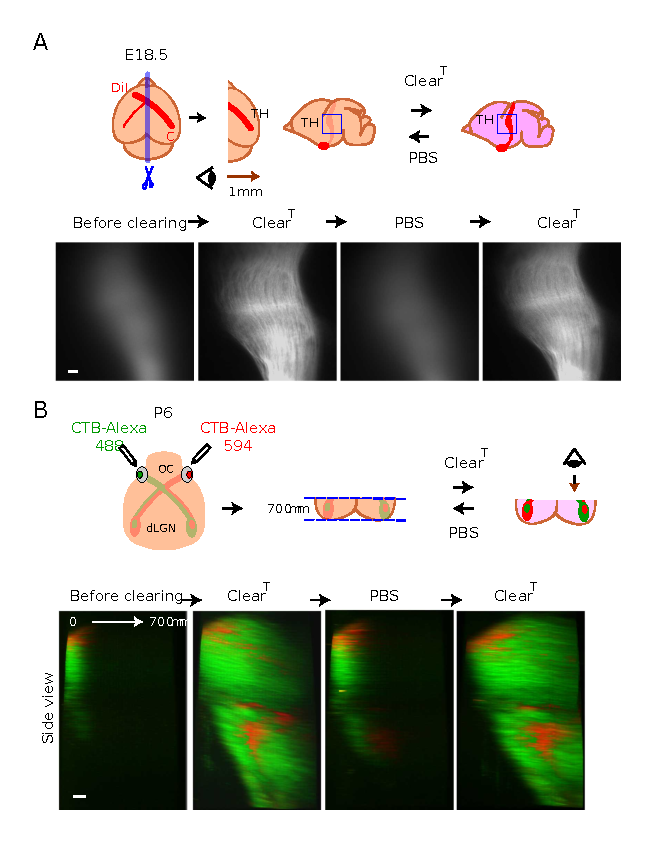
\includegraphics{Figures/ClearT_SFig3.pdf}
        \caption[Tissue can be repeatedly cleared with \emph{Clear\textsuperscript{T}}.]
        {Tissue can be repeatedly cleared with \emph{Clear\textsuperscript{T}}.
        A) E18.5 DiI-labeled brains were cleared with \emph{Clear\textsuperscript{T}} and returned to opacity in PBS, then cleared again with \emph{Clear\textsuperscript{T}}, again rendering the retinal projection in the upper optic tract apparent on the surface of the thalamus.
        B) A 700$\mu$m frontal section through the thalamus was re-cleared with \emph{Clear\textsuperscript{T}} after being returned to opacity in PBS, enabling eye-specific projections to be clearly seen in the dLGN.
        The micrographs are merged stacks of 71 images (10$\mu$m steps) of CTB-labeled retinal axon projections in the P6 dLGN, taken through a 5X objective.
        Scale bars=100$\mu$m.
        }
        \label{ClearTSFig3}
    \end{center}
\end{figure}
